\section{Classificação das rochas sedimentares}

As rochas sedimentares podem ser agrupadas, em uma primeira aproximação, de acordo com
a origem do material que as constitui:

\begin{enumerate}
  \item \textbf{siliciclásticas}: formadas predominantemente por fragmentos de minerais
        silicáticos e de rochas preexistentes;
  \item \textbf{carbonáticas}: constituídas principalmente por minerais carbonáticos,
        frequentemente com participação biogênica;
  \item \textbf{químicas}: originadas por precipitação a partir de soluções, incluindo
        evaporitos compostos por sulfatos e cloretos;
  \item \textbf{orgânicas ou biogênicas}: formadas pelo acúmulo de matéria orgânica ou de
        restos produzidos por organismos;
  \item \textbf{vulcanoclásticas}: constituídas por fragmentos de origem vulcânica.
\end{enumerate}

Esta seção concentra-se nas rochas siliciclásticas, tema predominante nas anotações da
disciplina.

\subsection{Conglomerados e brechas}

Conglomerados e brechas são rochas siliciclásticas cuja fração dominante inclui clastos
maiores que \SI{2}{\milli\metre}. Em uso descritivo, o termo \emph{conglomerado} costuma
ser aplicado a rochas com clastos predominantemente arredondados, enquanto
\emph{brecha} indica clastos predominantemente angulosos
\parencite{wentworth1922,nichols2009}.

\subsubsection{Composição dos clastos}

Quanto à diversidade litológica, podem ser usados os seguintes termos:

\begin{itemize}
  \item \textbf{monomítico}: predomínio de uma única litologia de clasto;
  \item \textbf{oligomítico}: pequena variedade de litologias;
  \item \textbf{polimítico}: presença de várias litologias.
\end{itemize}

\subsubsection{Suporte e matriz}

Nos conglomerados \textbf{clasto-suportados}, os clastos grossos se tocam e formam a
estrutura resistente da rocha. Nos conglomerados \textbf{matriz-suportados}, os clastos
ficam dispersos em uma matriz mais fina. Os termos \emph{ortoconglomerado} e
\emph{paraconglomerado} são usados, respectivamente, para esses dois arranjos, embora a
descrição direta do tipo de suporte seja mais clara \parencite{nichols2009}.

Uma denominação textural mais completa considera as proporções relativas de cascalho,
areia e lama. Assim, podem ocorrer termos como conglomerado arenoso, conglomerado
lamoso, arenito conglomerático e pelito conglomerático. O nome deve indicar primeiro a
fração subordinada e, por último, a fração dominante.

O diagrama da Figura~\ref{fig:classificacao-conglomerados} permite determinar essa
denominação a partir das porcentagens de cascalho, areia e lama.

\begin{figure}[H]
  \centering
  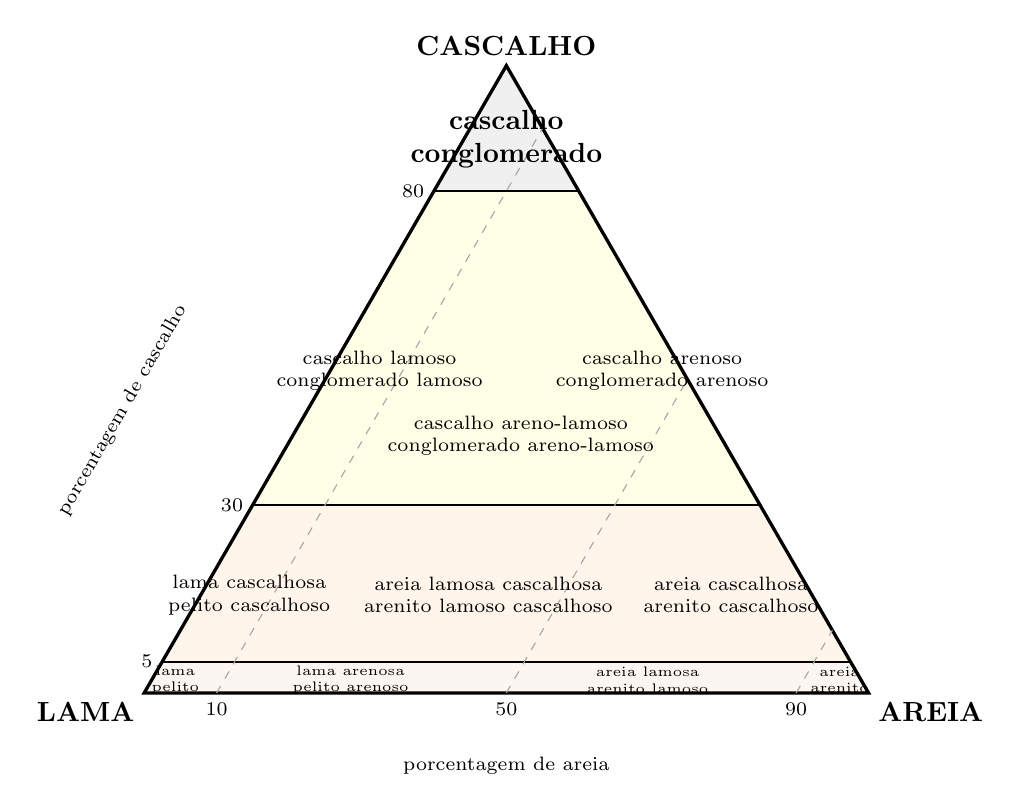
\begin{tikzpicture}[x=0.92cm,y=0.92cm,font=\scriptsize]
    \coordinate (M) at (0,0);
    \coordinate (S) at (10,0);
    \coordinate (G) at (5,8.66);

    % Campos granulométricos principais
    \path[fill=brown!7] (M)--(S)--(9.75,0.433)--(0.25,0.433)--cycle;
    \path[fill=orange!8] (0.25,0.433)--(9.75,0.433)--(8.5,2.598)--(1.5,2.598)--cycle;
    \path[fill=yellow!10] (1.5,2.598)--(8.5,2.598)--(6,6.928)--(4,6.928)--cycle;
    \path[fill=gray!12] (4,6.928)--(6,6.928)--(G)--cycle;

    % Contorno e limites de porcentagem de cascalho
    \draw[very thick] (M)--(S)--(G)--cycle;
    \draw[thick] (0.25,0.433)--(9.75,0.433); % 5% cascalho
    \draw[thick] (1.5,2.598)--(8.5,2.598);   % 30% cascalho
    \draw[thick] (4,6.928)--(6,6.928);       % 80% cascalho

    % Limites de porcentagem de areia
    \draw[gray!70,dashed] (1,0)--(5.5,7.794);   % 10% areia
    \draw[gray!70,dashed] (5,0)--(7.5,4.330);   % 50% areia
    \draw[gray!70,dashed] (9,0)--(9.5,0.866);   % 90% areia

    % Polos e eixos
    \node[above,font=\bfseries] at (G) {CASCALHO};
    \node[below left,font=\bfseries] at (M) {LAMA};
    \node[below right,font=\bfseries] at (S) {AREIA};
    \node[rotate=60] at (-0.30,3.9) {porcentagem de cascalho};
    \node[below] at (5,-0.75) {porcentagem de areia};
    \node[left] at (0.25,0.433) {5};
    \node[left] at (1.5,2.598) {30};
    \node[left] at (4,6.928) {80};
    \node[below] at (1,0) {10};
    \node[below] at (5,0) {50};
    \node[below] at (9,0) {90};

    % Nomenclatura das misturas
    \node[align=center,font=\bfseries] at (5,7.65)
      {cascalho\\conglomerado};

    \node[align=center] at (3.25,4.45)
      {cascalho lamoso\\conglomerado lamoso};
    \node[align=center] at (5.20,3.55)
      {cascalho areno-lamoso\\conglomerado areno-lamoso};
    \node[align=center] at (7.15,4.45)
      {cascalho arenoso\\conglomerado arenoso};

    \node[align=center] at (1.45,1.35)
      {lama cascalhosa\\pelito cascalhoso};
    \node[align=center] at (4.75,1.35)
      {areia lamosa cascalhosa\\arenito lamoso cascalhoso};
    \node[align=center] at (8.10,1.35)
      {areia cascalhosa\\arenito cascalhoso};

    \node[align=center,font=\tiny] at (0.43,0.18) {lama\\pelito};
    \node[align=center,font=\tiny] at (2.85,0.18) {lama arenosa\\pelito arenoso};
    \node[align=center,font=\tiny] at (6.95,0.18) {areia lamosa\\arenito lamoso};
    \node[align=center,font=\tiny] at (9.60,0.18) {areia\\arenito};
  \end{tikzpicture}
  \caption{Classificação textural de sedimentos e rochas formados por misturas de
  cascalho, areia e lama. Os limites de 5, 30 e 80\% referem-se à proporção de
  cascalho.}
  \label{fig:classificacao-conglomerados}
  \caption*{\footnotesize Fonte: adaptado de \textcite{nichols2009}.}
\end{figure}


\subsubsection{Imbricação}

Clastos alongados ou achatados podem apresentar orientação preferencial, denominada
\textbf{imbricação}. Quando interpretada juntamente com a geometria do depósito e outras
estruturas, essa orientação pode fornecer a direção da paleocorrente.

\subsection{Arenitos}

A classificação petrográfica dos arenitos utiliza a composição dos grãos do arcabouço e
a proporção de matriz. Os três polos composicionais usuais são:

\begin{itemize}
  \item \textbf{Q}: quartzo;
  \item \textbf{F}: feldspatos;
  \item \textbf{L}: fragmentos líticos.
\end{itemize}

No esquema adotado por Nichols, baseado em classificações clássicas, uma rocha com
menos de aproximadamente 15\% de matriz é uma \textbf{arenita}; entre aproximadamente
15\% e 75\% de matriz, é uma \textbf{wacke}. A composição Q--F--L permite subdividir as
arenitas em quartzoarenitos, subarcóseos, arcóseos, sublitoarenitos e litoarenitos; as
wackes podem ser quartzosas, feldspáticas ou líticas
\parencite{dott1964,nichols2009}.

A Figura~\ref{fig:classificacao-arenitos-prisma} reúne os dois critérios em um único
esquema tridimensional: a posição ao longo do prisma representa o teor de matriz,
enquanto cada face triangular representa as proporções normalizadas de Q, F e L.

\begin{figure}[H]
  \centering
  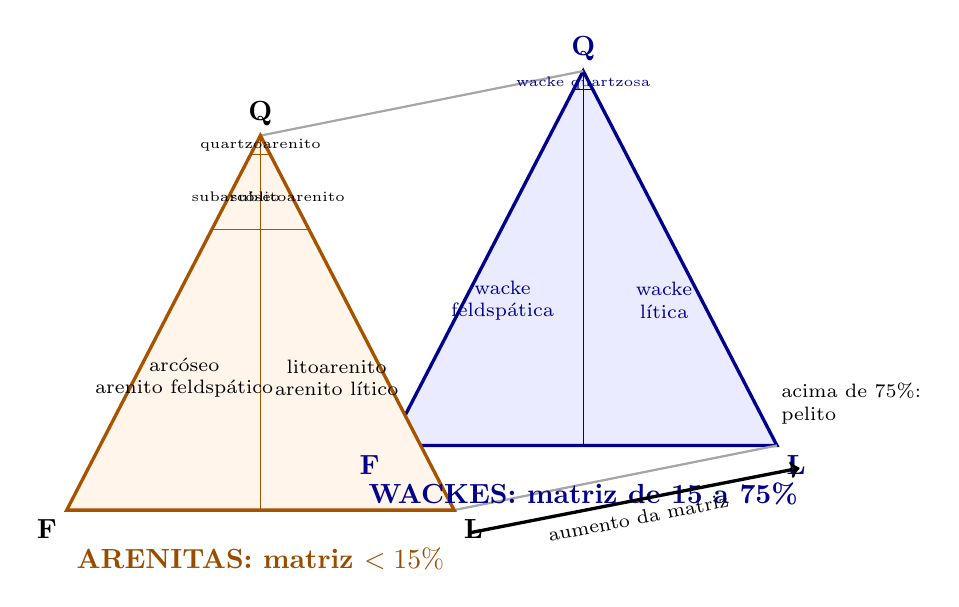
\begin{tikzpicture}[x=0.82cm,y=0.82cm,font=\scriptsize]
    % Triângulo posterior: wackes
    \coordinate (Qb) at (5,6.8);
    \coordinate (Fb) at (2,1.0);
    \coordinate (Lb) at (8,1.0);
    \path[fill=blue!8] (Qb)--(Fb)--(Lb)--cycle;
    \draw[very thick,blue!55!black] (Qb)--(Fb)--(Lb)--cycle;
    \draw[blue!55!black] (Qb)--(5,1.0);
    \draw[blue!55!black] (4.85,6.51)--(5.15,6.51);

    % Arestas que formam o prisma triangular
    \draw[gray!70,thick] (0,5.8)--(Qb);
    \draw[gray!70,thick] (-3,0)--(Fb);
    \draw[gray!70,thick] (3,0)--(Lb);

    % Triângulo anterior: arenitos/arenitas
    \coordinate (Q) at (0,5.8);
    \coordinate (F) at (-3,0);
    \coordinate (L) at (3,0);
    \path[fill=orange!8] (Q)--(F)--(L)--cycle;
    \draw[very thick,orange!65!black] (Q)--(F)--(L)--cycle;
    \draw[orange!65!black] (-0.15,5.51)--(0.15,5.51); % Q = 95%
    \draw[orange!65!black] (-0.75,4.35)--(0.75,4.35); % Q = 75%
    \draw[orange!65!black] (Q)--(0,0);                % F = L

    % Polos composicionais
    \node[above,font=\bfseries] at (Q) {Q};
    \node[below left,font=\bfseries] at (F) {F};
    \node[below right,font=\bfseries] at (L) {L};
    \node[above,font=\bfseries,text=blue!55!black] at (Qb) {Q};
    \node[below left,font=\bfseries,text=blue!55!black] at (Fb) {F};
    \node[below right,font=\bfseries,text=blue!55!black] at (Lb) {L};

    % Campos das arenitas
    \node[align=center,font=\tiny] at (0,5.65) {quartzoarenito};
    \node[align=center,font=\tiny] at (-0.38,4.85) {subarcóseo};
    \node[align=center,font=\tiny] at (0.42,4.85) {sublitoarenito};
    \node[align=center] at (-1.18,2.05) {arcóseo\\arenito feldspático};
    \node[align=center] at (1.18,2.05) {litoarenito\\arenito lítico};
    \node[font=\bfseries,orange!60!black] at (0,-0.75)
      {ARENITAS: matriz $<15\%$};

    % Campos das wackes
    \node[align=center,font=\tiny,text=blue!55!black] at (5,6.62)
      {wacke quartzosa};
    \node[align=center,text=blue!55!black] at (3.75,3.25)
      {wacke\\feldspática};
    \node[align=center,text=blue!55!black] at (6.25,3.25)
      {wacke\\lítica};
    \node[font=\bfseries,blue!55!black] at (5,0.25)
      {WACKES: matriz de 15 a 75\%};

    % Terceira dimensão do esquema
    \draw[->,very thick] (3.25,-0.35)--(8.35,0.65)
      node[midway,below,sloped] {aumento da matriz};
    \node[align=left] at (9.15,1.65) {acima de 75\%:\\pelito};
  \end{tikzpicture}
  \caption{Classificação prismática dos arenitos pelo teor de matriz e pela
  composição Q--F--L do arcabouço: Q = quartzo, F = feldspatos e
  L = fragmentos líticos.}
  \label{fig:classificacao-arenitos-prisma}
  \caption*{\footnotesize Fonte: adaptado da classificação de Pettijohn apresentada
  por \textcite{nichols2009}.}
\end{figure}


\subsection{Pelitos}

O termo \textbf{pelito} abrange rochas siliciclásticas de granulação fina. Conforme a
fração dominante e a fissilidade, podem ser usados os termos:

\begin{itemize}
  \item \textbf{siltito}: predomínio de partículas do tamanho silte;
  \item \textbf{argilito}: predomínio da fração argila, sem fissilidade marcante;
  \item \textbf{lamito}: mistura de silte e argila;
  \item \textbf{folhelho}: rocha fina com fissilidade, isto é, tendência a se separar em
        lâminas aproximadamente paralelas à estratificação.
\end{itemize}

\subsection{Maturidade textural e composicional}

A \textbf{maturidade textural} é avaliada principalmente pela quantidade de matriz, pelo
grau de seleção e pelo arredondamento. A \textbf{maturidade composicional} expressa a
proporção de componentes estáveis, sobretudo quartzo, em relação a componentes menos
estáveis, como feldspatos e determinados fragmentos líticos. As duas maturidades são
relacionadas à história sedimentar, mas não devem ser tratadas como sinônimos.
